\documentclass[14pt]{beamer}
\usetheme{Frankfurt}
\usepackage[utf8]{inputenc}
\usepackage[russian]{babel}
\usepackage[OT1]{fontenc}
\usepackage{amsmath}
\usepackage{amsfonts}
\usepackage{amssymb}
\usepackage{graphicx}
\author{Garifullin Albert}
\title{Компактное представление большой группы процедурно созданных деревьев}
%\setbeamercovered{transparent} 
%\setbeamertemplate{navigation symbols}{} 
%\logo{} 
%\institute{} 
%\date{} 
%\subject{} 
\begin{document}

\begin{frame}
\titlepage
\end{frame}

%\begin{frame}
%\tableofcontents
%\end{frame}
  
\begin{frame}{Проблемы процедурной генерации}
 - Использовать много уникальных моделей напрямую не позволяют ограничения
   памяти\linebreak	
 - Использование небольшого числа заранее подготовленных моделей не обеспечивает желаемого разнообразия\linebreak	
 
 Как сохранить реалистичность и разнообразие процедурно генерируемых растений без необходимости хранить детализированные модели?
\end{frame}
\begin{frame}{Кластеризация}

По множеству уникальных деревьев построить набор базовых структурных элементов, из которых, используя простые геометрические преобразования, можно получить деревья, внешне минимально отличающиеся от исходных.
\end{frame}
\begin{frame}{Кластеризация}
Дерево представляется как структура, состоящая из ствола и веток, растущих из него. \linebreak	
Множетства все стволов и веток множества деревьев по отдельности проходят процедуру кластеризации - разделение на группы структурно похожих между собой элементов.\linebreak	
Все элементы одного кластера заменяются на instance типичного представителя\linebreak	
Для создания импостеров кластеризации подвергается само множество деревьев\linebreak	
\end{frame}
\begin{frame}{Кластеризация}
\begin{figure}[hbtp]
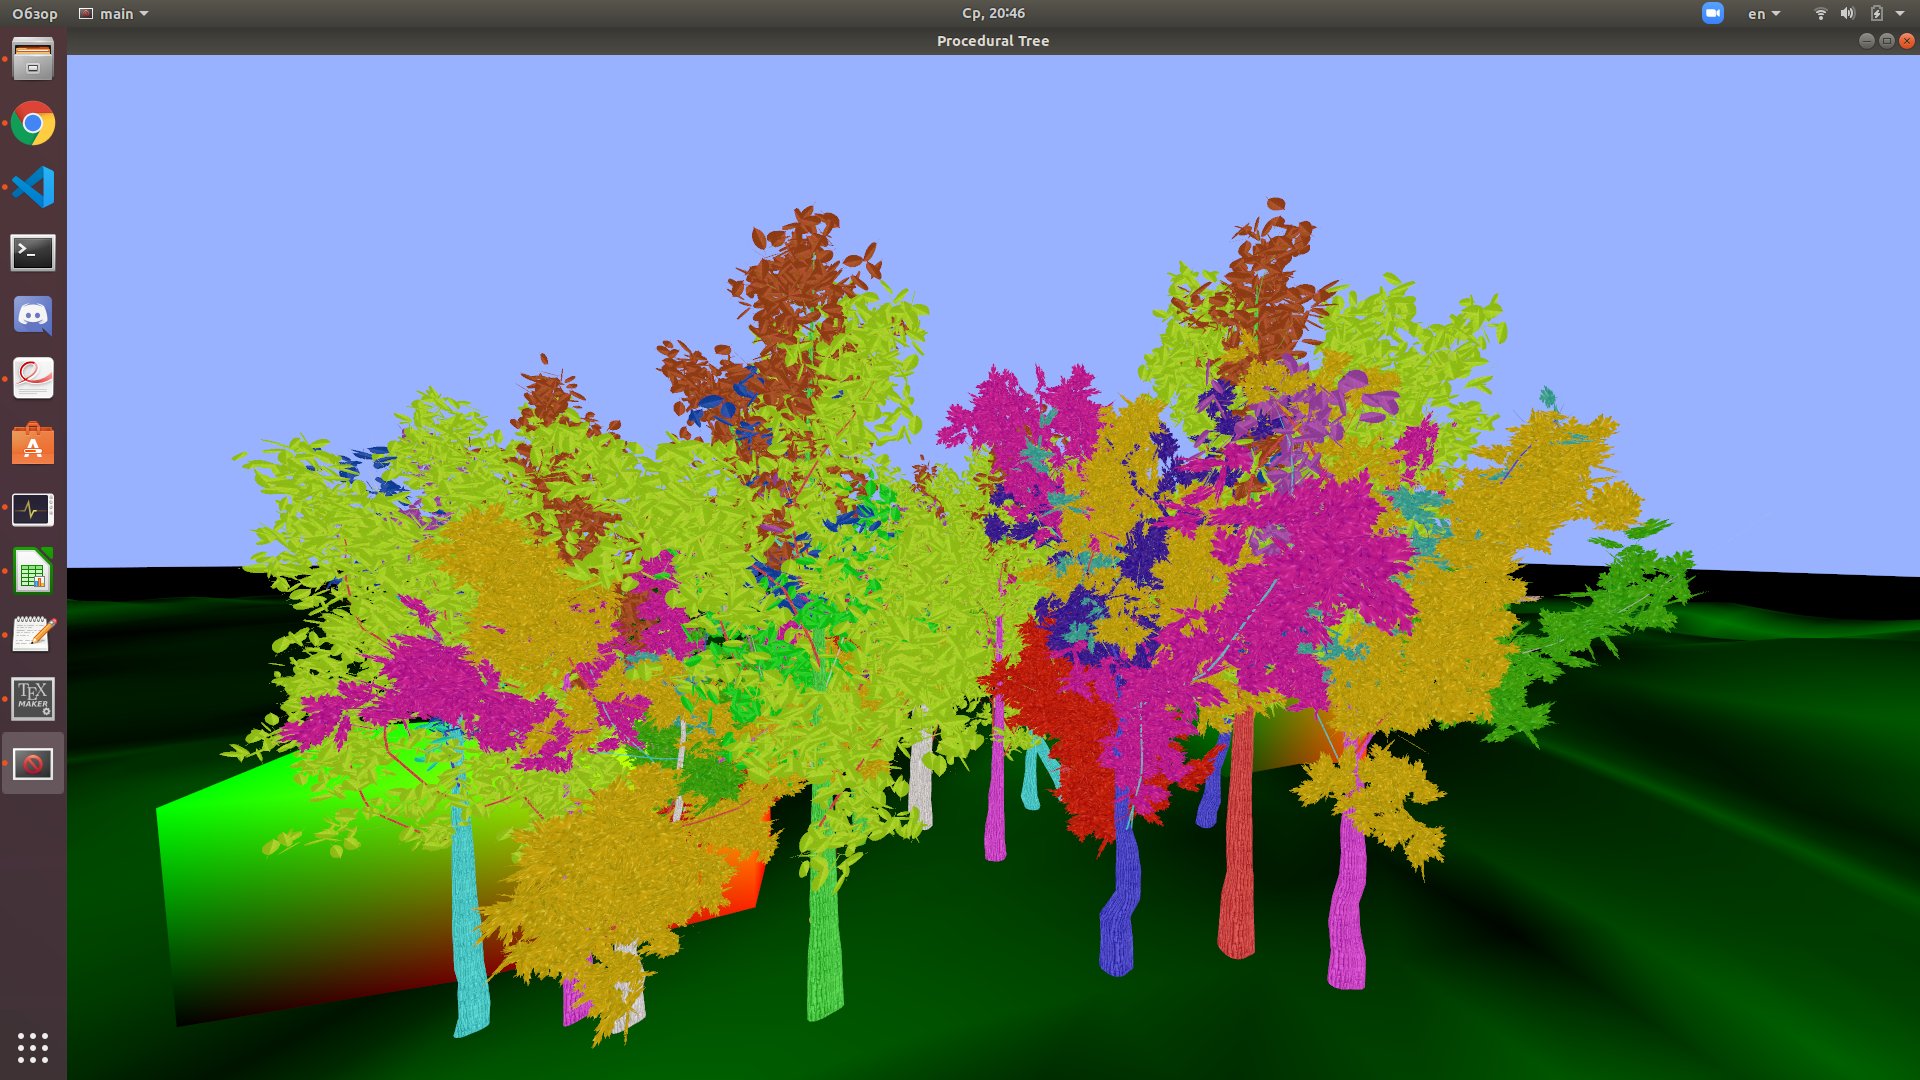
\includegraphics[scale=0.165]{clusters.png}
\end{figure}
\end{frame}
\begin{frame}{Оригинальная группа деревьев}
\begin{figure}[hbtp]
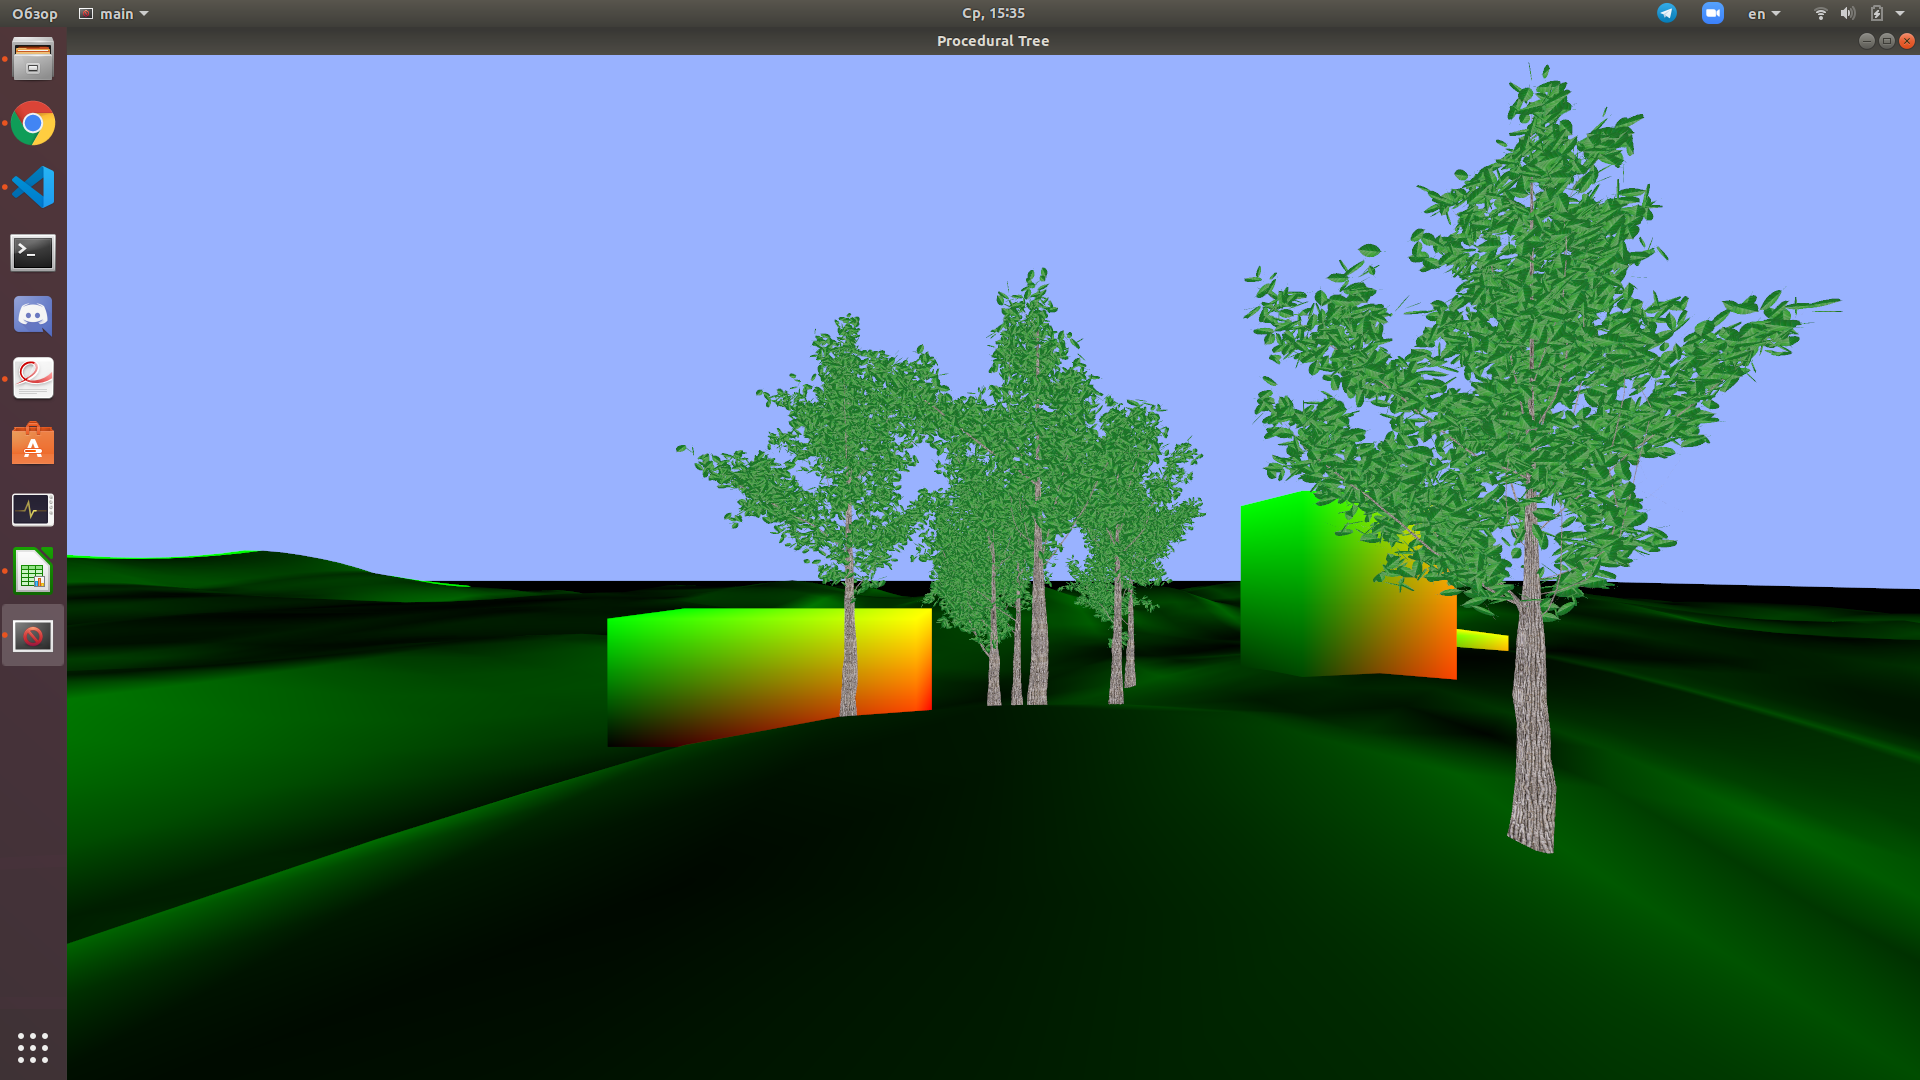
\includegraphics[scale=0.165]{92_clusters.png}
\end{figure}
\end{frame}
\begin{frame}{20 кластеров}
\begin{figure}[hbtp]
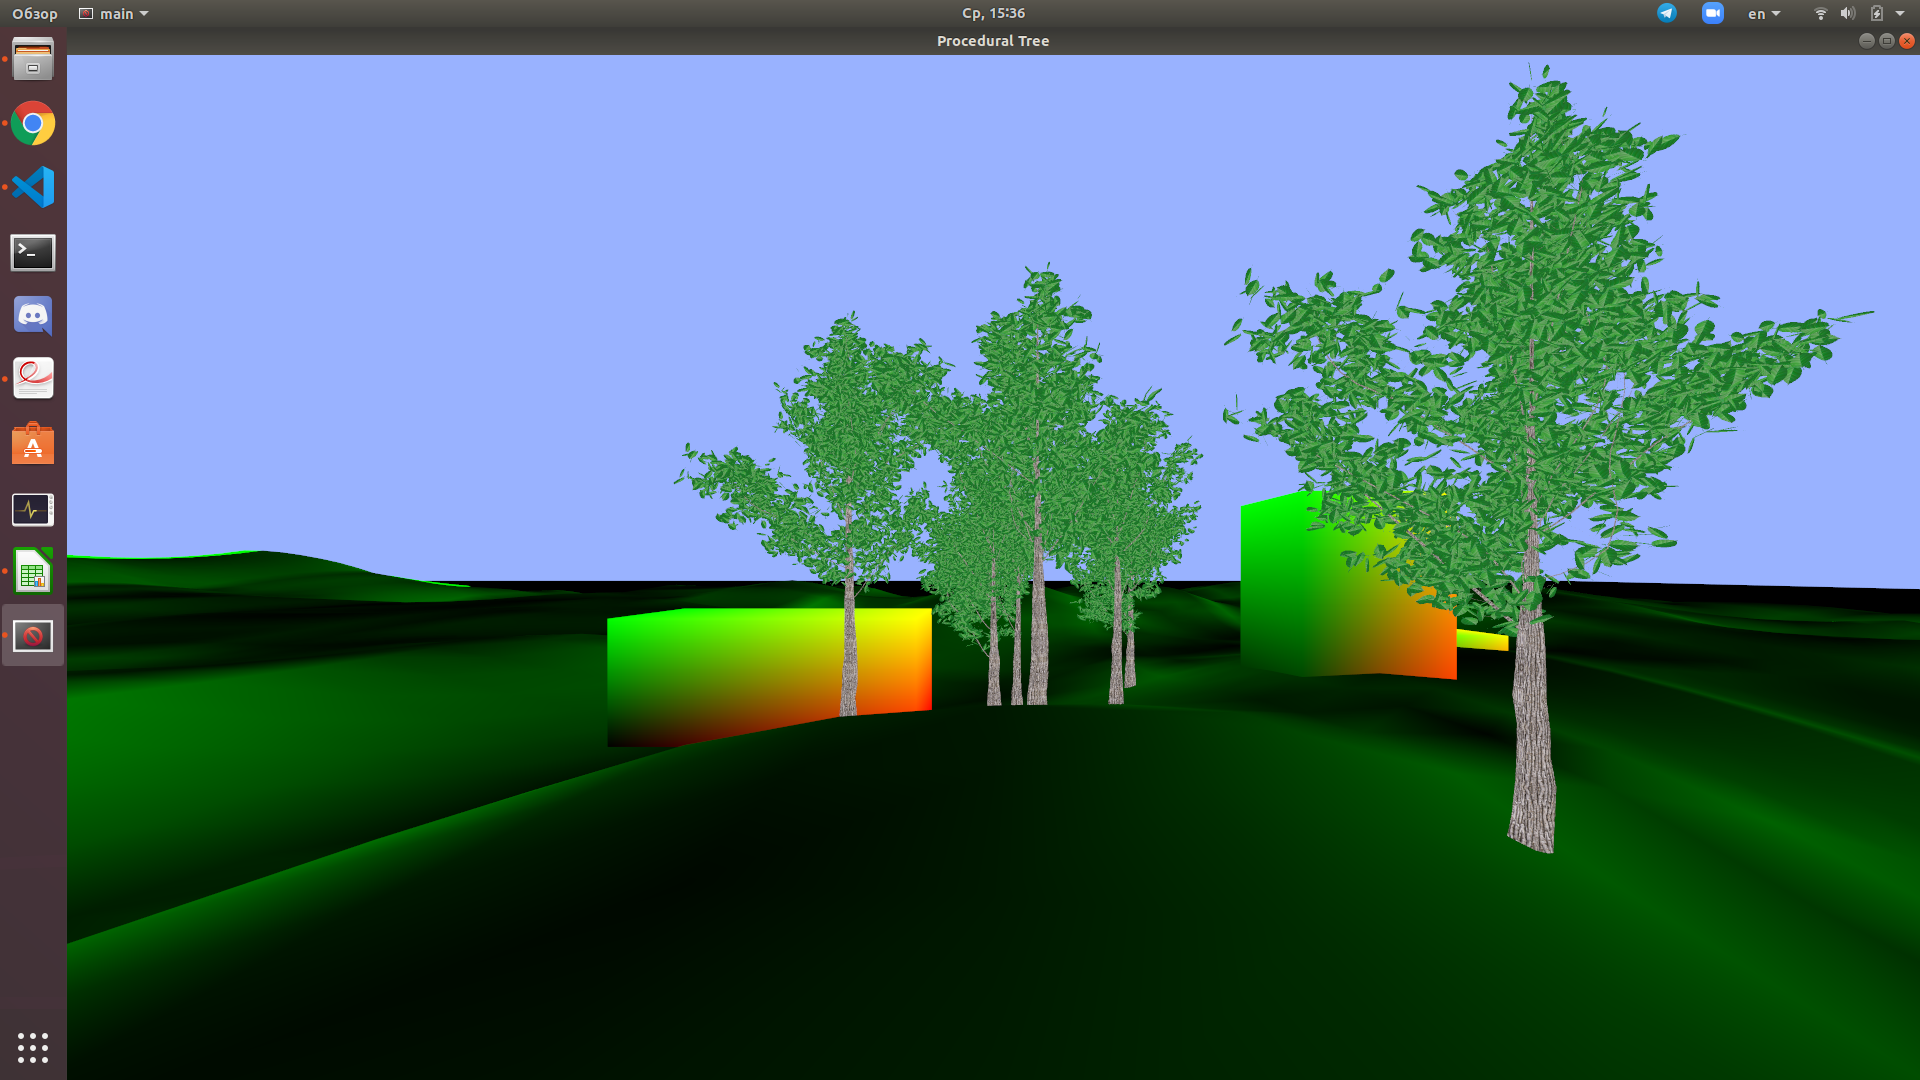
\includegraphics[scale=0.165]{20_clusters.png}
\end{figure}
\end{frame}
\begin{frame}{1 кластер}
\begin{figure}[hbtp]
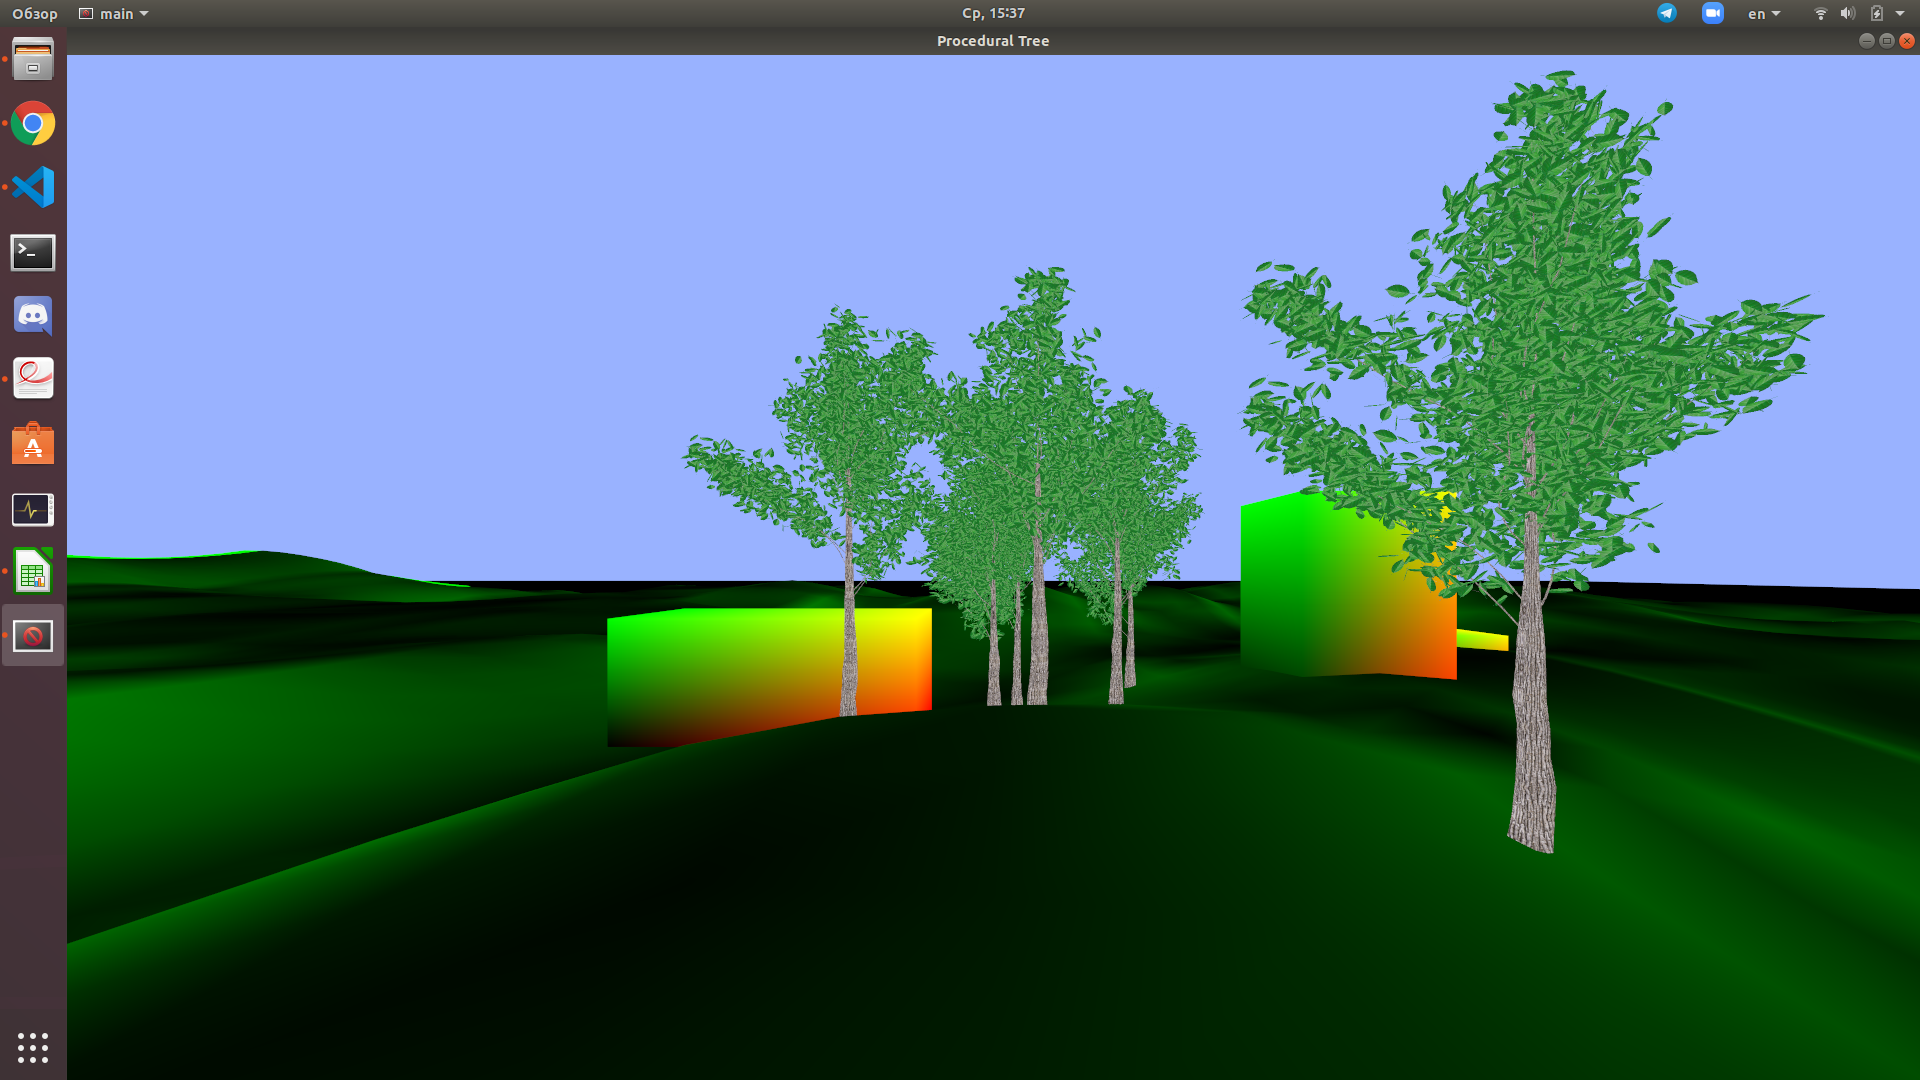
\includegraphics[scale=0.165]{1_cluster.png}
\end{figure}
\end{frame}
\begin{frame}{Кластеризация}
MID - максимальная индивидуальная дистанция между элементами
кластера 
Эффективность повышается при увеличении числа объектов в исходной группе
\begin{figure}[hbtp]
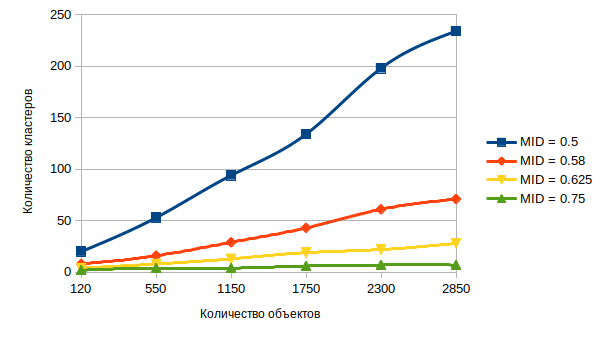
\includegraphics[scale=0.58]{stat2.png}
\end{figure}
\end{frame}
\begin{frame}{Кластеризация}
\begin{figure}[hbtp]
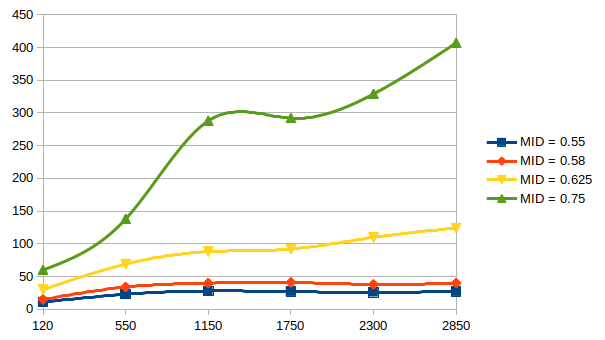
\includegraphics[scale=0.6]{stat3.png}
\end{figure}
\end{frame}
\begin{frame}{Синтетические деревья}
1) Создаем относительно небольшую группу деревьев генератором\linebreak	
2) Проводим кластеризацию\linebreak	
3) Собираем статистику о параметрах кластеризованных деревьев\linebreak	
4) На основании нее синтезируем новые матрицы трансформации для существующих кластеров, которые формируют новые, "синтетические" деревья
\end{frame}
\begin{frame}{Эффективность}
На 1 кластер уходит 5-15\% от памяти, необходимой для хранения всего дерева\linebreak	
На изображении ниже 27 кластеров и 11 импостеров на 1250 уникальных деревьев. \linebreak	
\begin{figure}[hbtp]
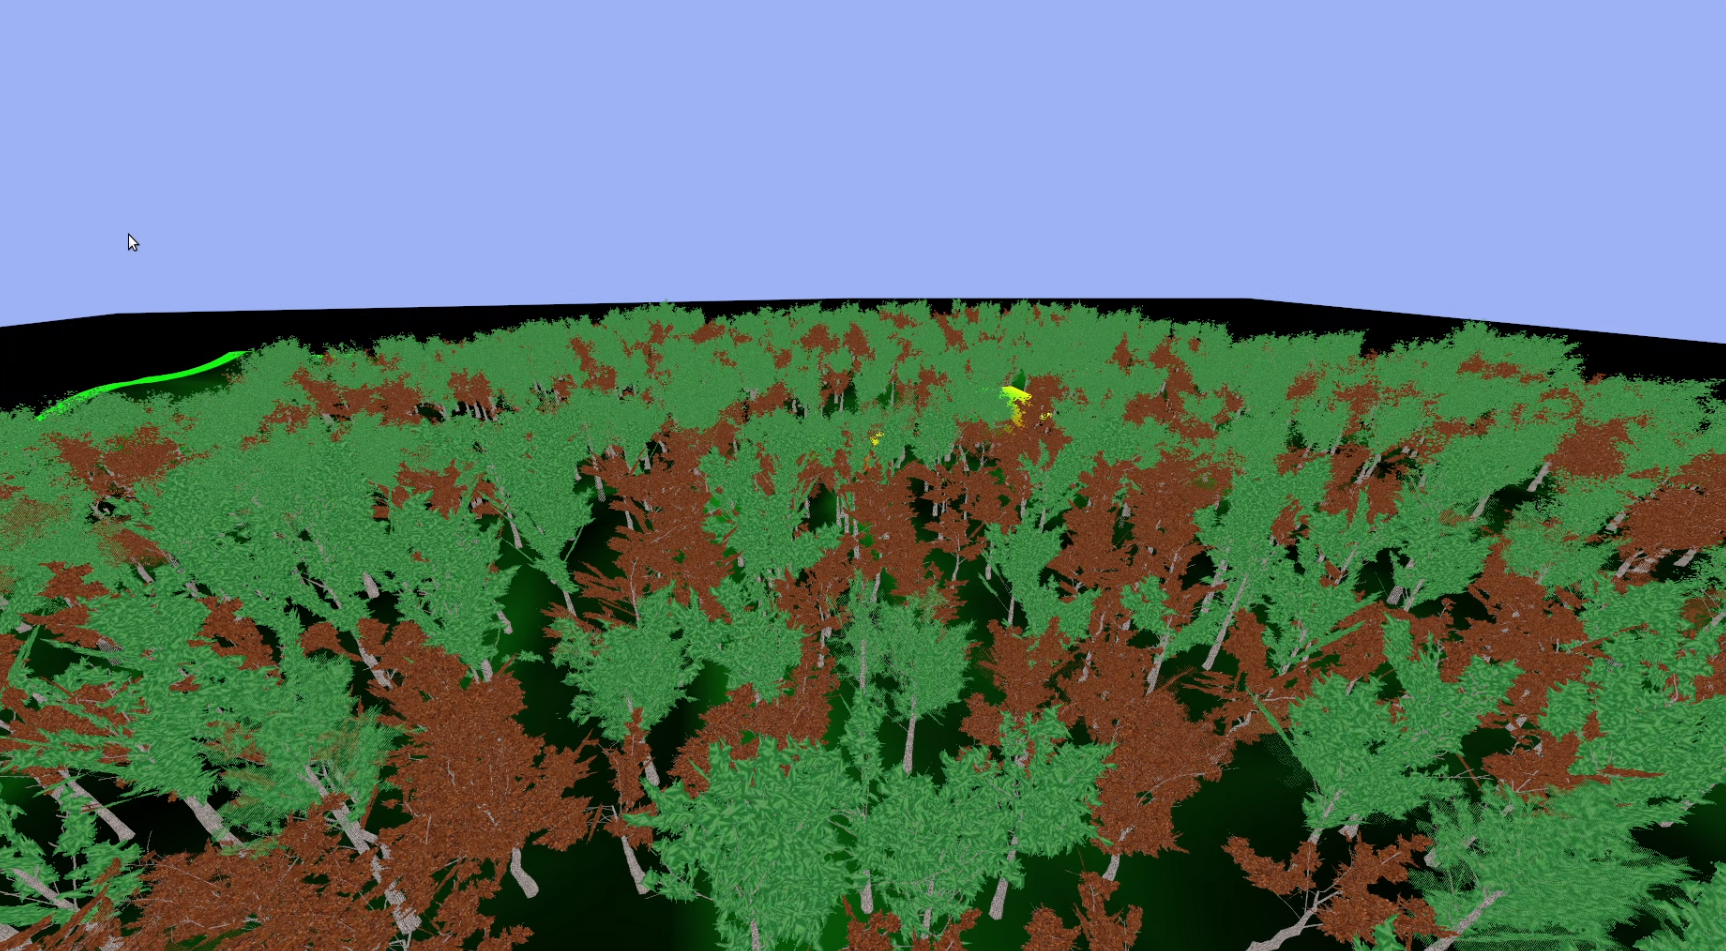
\includegraphics[scale=0.137]{large.png}
\end{figure}
\end{frame}
\begin{frame}{Преимущества}
1) Сохраняется уникальность деревьев и, в целом, их форма и структура, заложенная генератором на основе внутренней логики (физическая симуляция, внутриигровая логика)\linebreak	
\end{frame}
\begin{frame}{Преимущества}
2) Процедура кластеризации не завязана на конкретный генератор деревьев
Может использоваться любой генератор, если результат его работы будет конвертирован в структурное представление дерева, необходимое для кластеризации\linebreak	
\end{frame}
\begin{frame}{Преимущества}
3) Результатом работы алгоритма являются структуры данных, типичные для описания растительности на сцене - набор моделей (биллбордов, импостеров) и списки матриц трансформаций их instance'ов. Для их рендера можно использовать уже существующие алгоритмы.
\end{frame}
\begin{frame}{Недостатки}
1) Алгоритм применяется ко всей группе целиком и не допускает процедурную генерацию в real-time \linebreak	
2) Из-за того, что минимальной единицей для рендера является ветка, а не дерево целиком, увеличивается расход ресурсов на операции, выполняемые для каждого instance - например, определение LOD'а.
\end{frame}
\begin{frame}{Вывод}
 - Реализован механизм преобразующий группу процедурно сгенерированных деревьев в набор базовых структурных элементов, из которых, используя простые геометрические преобразования, можно получить деревья, внешне минимально отличающиеся от исходных. \linebreak	
 - Также реализован алгоритм создания новых деревьев из полученных базовых элементов, по своему строению имитирующих исходные\linebreak
\end{frame}
\begin{frame}{Вывод}	
Все это дает возможность создавать сцены с большим числом уникальных растений с высокой детализацией с расходом ресурсов не больше, чем при стандартном подходе с несколькими заранее подготовленными моделями.
\end{frame}
\begin{frame}{Конец}
Спасибо за внимание!
\end{frame}
\end{document}